% Editorial condensation of Magenta_Gap_MSS(1).pdf (July 2026).
% See EDITORIAL_NOTES.md for substantive corrections and source provenance.
\documentclass[9pt,twocolumn,twoside]{opticajnl}
\journal{opticajournal}
\setboolean{shortarticle}{false}
\setboolean{displaycopyright}{false}
\doi{}
\usepackage{amsmath,amssymb,amsthm,mathtools}
\usepackage{graphicx,booktabs,microtype}
\hypersetup{pdftitle={Magenta gap: a geometric reachability model of nonspectral hue and color gamut boundaries},pdfauthor={Alexander Yiannopoulos}}
\theoremstyle{plain}
\newtheorem{proposition}{Proposition}
\newtheorem{theorem}[proposition]{Theorem}
\newcommand{\dd}{\mathrm{d}}
\newcommand{\R}{\mathbb{R}}
\title{Magenta gap: a geometric reachability model of nonspectral hue and color gamut boundaries}
\author[1,*]{Alexander Yiannopoulos}
\affil[1]{A$\lvert\Omega\rangle$ Institute, Alpha Omega Lattice Corporation, 3724 Laurel Street, Suite 108, New Orleans, Louisiana, USA}
\affil[*]{ayianno@ao.institute}
\begin{abstract}
Monochromatic stimuli are ordered by wavelength, whereas hue includes a nonspectral purple closure. We model this closure by inserting a purple interval into a compactified spectral arc, then incorporate the resulting hue circle into a color body with an achromatic quotient. A proposed indefinite reachability metric makes a prescribed gamut boundary piecewise null. Under explicit calibration and regularity assumptions, nullity bounds the angular variation of the saturation ceiling; a diagonal construction requires strict inequality. Cone-fundamental calculations illustrate the constraint's dependence on normalization and metric scale. The construction separates a geometric compatibility condition from the physiological assumptions needed for optical confinement.
\end{abstract}
\begin{document}
\maketitle

\section{Introduction}
\label{sec:introduction}
Color perception provides a concrete setting in which physical stimulus coordinates, color-matching relations, and the organization of appearance must be distinguished. Wavelength orders monochromatic stimuli along a line. Hue, by contrast, includes a route from violet to red through the nonspectral purples. Magenta has no single-wavelength correlate, although it is induced by physically ordinary spectral mixtures. The resulting ``magenta gap'' concerns the organization of a response space, rather than an absent physical wavelength.

Geometrical approaches to color have a substantial history. Color-matching structure is formalized by Grassmann representations \cite{Krantz1975}; differential-geometric models address additional questions about color-space organization and discrimination \cite{Resnikoff1974}. Appearance also depends on adaptation, surround, and the viewing regime \cite{Shevell2003,Fairchild2013}. A physical account therefore begins with spectral distributions and an observer-dependent response map, not with an identification of color and wavelength. The wavelength interval is only a restricted locus within the full stimulus domain.

This paper develops a geometric model in three stages. First, the ordered spectral arc is completed by a purple interval to form a resolved hue circle. Second, hue is collapsed at zero chromatic radius, giving a three-dimensional color body with an achromatic axis. Third, an indefinite metric is introduced as a \emph{reachability gauge}: a device for representing a prescribed boundary of ordinary optical access. The metric is not a perceptual-distance function, and its signature does not follow from the topology. It is a further modeling assumption whose mathematical consequences can be stated separately from its physiological interpretation.

The principal result concerns a positive hue-dependent ceiling $\alpha(\theta)$ and the boundary
\begin{equation}
 R(\theta,z)=\alpha(\theta)(T-|z|).
 \label{eq:boundary-intro}
\end{equation}
If each open sheet is null for the calibrated metric specified below, with positive-definite spatial block, then
\begin{equation}
 \left|\frac{\dd\log\alpha}{\dd\theta}\right|\leq\beta(\theta,z),
 \label{eq:bound-intro}
\end{equation}
where $\beta$ is the boundary angular metric scale divided by its chromatic radius. The inequality is covariant under reparameterization of hue. A finite positive radial coefficient in the diagonal construction requires strict inequality. These statements constrain the compatibility of a boundary and a chosen metric; they do not independently establish either as a description of human vision.

The distinction is consequential. The bicone shape and its calibration are inputs, not predictions derived from cone physiology. Its equatorial ridge follows from the assumed symmetric shape. A related obstruction to a smooth null radial envelope holds under explicit metric and boundary hypotheses. Neither statement proves that optical response trajectories are confined by the metric. We therefore separate the geometry, a numerical consistency calculation using cone fundamentals, and the additional control condition that a reachability interpretation would require.

\section{Spectral stimuli and resolved hue}
\label{sec:hue}
\subsection{Stimulus space and nonspectrality}
Let $a$ denote an observer and fixed viewing regime, including the adaptation and surround conditions relevant to the response. Let $\mathcal S_a$ be an admissible cone of finite positive spectral measures, and let
\begin{equation}
 \Phi_a:\mathcal S_a\longrightarrow M_a
 \label{eq:response}
\end{equation}
be its response map. Measures accommodate both continuous spectral power distributions and idealized monochromatic stimuli. The latter have the form $t\delta_\lambda$, where $t>0$ specifies intensity. After choosing an intensity normalization, the wavelength interval
\begin{equation}
 I_a=(\lambda_-^a,\lambda_+^a)
 \label{eq:interval}
\end{equation}
parametrizes a one-dimensional stimulus locus. The endpoints are ideal limiting directions of the chosen model; finite numerical cutoffs are experimental or computational proxies.

The map $\Phi_a$ induces a metameric relation,
\begin{equation}
 \mu\sim_a\nu\quad\Longleftrightarrow\quad\Phi_a(\mu)=\Phi_a(\nu).
 \label{eq:metamerism}
\end{equation}
A response class is spectral when it contains a monochromatic representative $t\delta_\lambda$ under the stated regime and permitted intensity range. A nonspectral class contains none. This is a condition on the preimage of the response map. It does not deny the physical causation of nonspectral responses, and it does not make the entire stimulus space one-dimensional. For a hue-only classification, the same definition is applied after the appropriate appearance coordinates have been fixed or projected out.

Human purple responses are paradigmatically induced by mixtures with short- and long-wavelength contributions. A mixture coordinate is consequently a response-side or colorimetric coordinate, not a wavelength between red and violet. The actual relation between mixture weights and hue depends on the observer and regime. The construction below records an ordered purple continuum without claiming that its parameter is perceptually uniform or directly proportional to radiant power.

We idealize the spectral hue responses used in the construction as an ordered arc. This is an explicit modeling restriction: the full spectral-response curve and its hue projection need not be globally injective in every regime. The interval gluing describes the intended hue organization once that arc and its limiting classes have been identified. It is not a theorem that all visual systems must implement this particular construction.

\subsection{Compactification and insertion of the purple interval}
Since an open bounded interval is homeomorphic to $\R$, its one-point compactification is a circle,
\begin{equation}
 H_a=\widehat I_a=I_a\cup\{\infty\}\cong S^1.
 \label{eq:compactification}
\end{equation}
The added point is an abstract closure marker. It is neither a wavelength nor an additional stimulus. Equivalently, $\widehat I_a$ is obtained from the auxiliary closed interval $\overline I_a$ by identifying its endpoints. This identifies the ends only in the auxiliary topological model; it does not identify the physical spectral directions.

To represent distinguishable purples, introduce $P_a=[0,1]$ and glue its endpoints to those of $\overline I_a$:
\begin{equation}
 \widetilde H_a=\overline I_a\cup_{\partial I_a}P_a\cong S^1,
 \qquad 0\sim\lambda_+^a,\quad 1\sim\lambda_-^a.
 \label{eq:gluing}
\end{equation}
Thus $\tau=0$ denotes the red-side limit and $\tau=1$ the violet-side limit of the purple interval. The spectral arc runs in the opposite direction, closing the circle. A collapse map records this insertion:
\begin{equation}
 \pi:\widetilde H_a\longrightarrow H_a,
 \qquad \pi^{-1}(\infty)=P_a.
 \label{eq:collapse}
\end{equation}
On the spectral interior, $\pi$ identifies the two copies of $I_a$. The endpoints of $P_a$ are attachment classes; its interior represents the nonspectral transition. Figure~\ref{fig:hue} summarizes the construction.

\begin{figure*}[t]
\centering
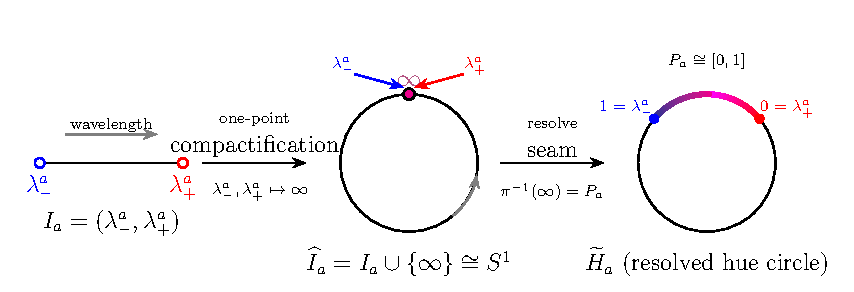
\includegraphics[width=0.83\textwidth]{fig1_magenta_gap.pdf}
\caption{Compactification and resolution of the modeled hue circle. The physical interval, its abstract one-point compactification, and the resolved response circle are distinct objects. Inserting $P_a$ represents the purple continuum without adding wavelengths. The closed interval includes the two attachment classes; its interior is the nonspectral arc. This is a structural model of hue organization, not a physiological derivation.}
\label{fig:hue}
\end{figure*}

The word ``resolution'' refers here to inserting an interval over the abstract seam. The compactification point is already a regular point of a circle; there is no mathematical singularity requiring a blow-up. The operation gives a way to retain the distinction between spectral and purple arcs within a common cyclic target space. Both arcs belong to the response model, but only the spectral arc is supplied with a wavelength parameter.

A smooth structure may be chosen on $\widetilde H_a$. Its existence does not imply that the raw wavelength coordinate and a chosen mixture coordinate have matching derivatives at the seams. Smooth charts require suitable local reparameterizations. The model therefore separates the topology of the glued circle from its angular calibration,
\begin{equation}
 \theta:\widetilde H_a\longrightarrow\R/(2\pi\mathbb Z).
 \label{eq:hue-angle}
\end{equation}
Changing this calibration transforms the metric components and derivatives used below. There is no preferred angular spacing determined by the gluing alone.

\section{Quotient color body and metric model}
\label{sec:body}
\subsection{The achromatic quotient}
Let $r\in[0,r_{\max}]$ denote a chromatic radius and $z\in L_a$ a centered luminosity coordinate. Neither is assumed at this stage to be a standardized perceptually uniform coordinate. Hue is undefined at $r=0$, so the ambient color body is modeled by
\begin{equation}
 M_a=\bigl([0,r_{\max}]\times\widetilde H_a\times L_a\bigr)/\sim,
 \qquad (0,h,z)\sim(0,h',z).
 \label{eq:quotient}
\end{equation}
The achromatic axis is $A_a=\{r=0\}$. Its points carry luminosity but no chromatic phase. On $M_a^*=M_a\setminus A_a$, the projection to $\widetilde H_a$ has local fiber coordinates $(r,z)$. This bundle description applies only to the chromatic stratum. Treating the entire body as a product with the hue circle would artificially assign every neutral state a family of hue labels.

Choosing $x=r\cos\theta$ and $y=r\sin\theta$ identifies the chromatic disk in ordinary Cartesian coordinates. A convenient baseline metric is
\begin{equation}
 g_0=\dd r^2+r^2\dd\theta^2-\kappa^2\dd z^2
     =\dd x^2+\dd y^2-\kappa^2\dd z^2,
 \qquad\kappa>0.
 \label{eq:baseline}
\end{equation}
The polar chart fails on the axis, but the Cartesian tensor is regular there. The period $2\pi$ is part of this coordinate convention. Under a nonlinear angular reparameterization, the component multiplying the new angular differential must transform; one cannot preserve the bare $r^2$ expression and simultaneously claim to have kept the same metric.

The gauge and a local discrimination metric are different objects. Choosing a regular Cartesian core for $g_0$ does not specify discrimination thresholds near gray, nor does it identify coordinate circumference with perceptual circumference. Empirical anisotropy may enter a separately calibrated discrimination tensor. The boundary identification used in Sec.~\ref{sec:numerics}.\ref{sec:identification} is an additional assumption linking that tensor to the reachability construction.

\subsection{Fixed-hue sections and the role of the signature}
Each fixed-hue radial--luminosity section has the quadratic form
\begin{equation}
 g_\theta=\dd r^2-\kappa^2\dd z^2.
 \label{eq:section-metric}
\end{equation}
It admits the split-complex notation $q=r+j\kappa z$, $j^2=1$, with $q\overline q=r^2-\kappa^2z^2$. The state-space section is a half-plane because $r\geq0$; its tangent-space quadratic form has signature $(1,1)$. This notation introduces no fourth color coordinate. Hue labels the section rather than contributing another component to $q$.

Hyperbolic rotations preserve the baseline split form. That algebraic fact does not establish that adaptation or luminance-induced changes in colorfulness follow such rotations. A connection to phenomena such as the Hunt effect would require a response model and an independent test. The present use of the split form is restricted to describing the proposed metric and its null directions.

The minus sign distinguishes the luminosity direction in the chosen reachability model. A null displacement is not asserted to be a zero perceptual difference. Likewise, a spacelike displacement is not inherently inaccessible: ordinary isoluminant changes have $\dd z=0$ and positive spatial norm. These facts prevent the metric alone from serving as a physiological rule for permitted transitions.

Work on non-Riemannian color differences further illustrates why a local discrimination model and a global appearance-distance model must be distinguished \cite{Bujack2022}. It does not supply affirmative evidence for the indefinite metric in Eq.~\eqref{eq:baseline}. Our metric requires its own justification through the boundary and control assumptions described below.

For a fixed ordinary regime $a_0$, write
\begin{equation}
 C_{a_0}=\operatorname{im}\Phi_{a_0}\subset M_{a_0}.
 \label{eq:image}
\end{equation}
The model assigns the ordinary optical image a spindle-like boundary. To compare it with another regime, both images must first be represented in a common calibrated ambient space. A change of adaptation may then change the response map and its image. The claim that an altered-regime percept lies outside the ordinary image is operational and requires such calibration; the drawing of an exterior region is not itself evidence for that claim.

\section{Null-boundary compatibility}
\label{sec:constraint}
\subsection{Symmetric normal form}
Take $L_{a_0}=[-T,T]$ with $T>0$. In the isotropic baseline, the prescribed body is
\begin{equation}
 C^{\mathrm{sym}}=\{(r,\theta,z):r\leq\kappa(T-|z|),\ |z|\leq T\}.
 \label{eq:bicone}
\end{equation}
It is the intersection of the two appropriately oriented cones from the achromatic poles $(0,0,\pm T)$. For example, a lower-sheet generator is
\begin{equation}
 \gamma_\theta(s)=(\kappa s\cos\theta,\kappa s\sin\theta,-T+s),
 \quad 0<s<T,
 \label{eq:generator}
\end{equation}
and $g_0(\dot\gamma_\theta,\dot\gamma_\theta)=\kappa^2-\kappa^2=0$. The upper sheet has the same property. They meet continuously with different $z$-slopes at $z=0$, as illustrated in Fig.~\ref{fig:spindle}.

\begin{figure}[t]
\centering
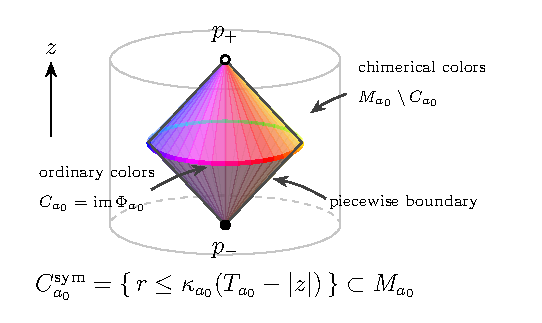
\includegraphics[width=0.96\linewidth]{fig3_spindle.pdf}
\caption{Prescribed symmetric reachability body inside the ambient color model. The open upper and lower sheets are null for the calibrated baseline metric and meet at an equatorial ridge. The equatorial location follows the assumed symmetry. Exterior points are candidates for comparison across viewing regimes; their physiological accessibility is not implied by the metric.}
\label{fig:spindle}
\end{figure}

This is a calibration of the metric to the chosen bicone. The linear narrowing toward the poles is not derived from a measurement of gamut shape. Consequently, observing an equatorial ridge would not by itself confirm the metric, and a general empirical color body is not required by topology to possess this ridge. The following narrower statement explains the obstruction within the radial-graph setting.

\begin{proposition}[Obstruction to a smooth null radial envelope]
\label{prop:ridge}
Suppose a compact radial-graph body has boundary $r=R(\theta,z)$ for $-T\leq z\leq T$, with $R(\theta,\pm T)=0$ and a positive interior value for some fixed $\theta$. Let the metric have no spatial--$z$ cross-terms and a positive-definite spatial block. Then the graph cannot be differentiable everywhere and null everywhere on its positive-radius part.
\end{proposition}
\begin{proof}
For the stated fixed hue, $R$ has a positive interior maximum in $z$. If the graph is differentiable there, $R_z=0$. With $F=r-R$, the conormal is $\dd F=(1,-R_\theta,0)$. Because the inverse spatial block is positive definite, $g^{-1}(\dd F,\dd F)>0$, contradicting nullity.
\end{proof}
The proposition uses the radial-graph and metric hypotheses. It forces a failure of differentiability somewhere if the entire boundary is to remain null; it does not locate that failure at an isoluminant equator for an arbitrary body. Equation~\eqref{eq:bicone} supplies that location through symmetry. The achromatic tips are separate singular points of the boundary graph.

\subsection{Hue-dependent ceiling and general spatial block}
Let $\alpha(\theta)>0$ be smooth and periodic, and prescribe Eq.~\eqref{eq:boundary-intro}. On either open sheet, away from the ridge and tips, consider
\begin{equation}
 \dd s^2=A\,\dd r^2+2D\,\dd r\,\dd\theta+B\,\dd\theta^2-C\,\dd z^2,
 \label{eq:metric}
\end{equation}
where $A>0$, $C>0$, and $\Delta=AB-D^2>0$. These conditions make the spatial block positive definite and give signature $(2,1)$. The absence of spatial--$z$ cross-terms is part of the ansatz. All coefficients below are evaluated on the boundary unless stated otherwise.

For $F=r-R(\theta,z)$, the null-conormal equation is
\begin{equation}
 \frac{B+2DR_\theta+AR_\theta^2}{\Delta}-\frac{R_z^2}{C}=0.
 \label{eq:null-general}
\end{equation}
The original model fixes the luminosity coefficient on the boundary by
\begin{equation}
 C=\alpha(\theta)^2.
 \label{eq:calibration}
\end{equation}
Since $R_z=\mp\alpha$ on the two sheets, $R_z^2/C=1$. This calibration is essential. Without it, the null condition relates the same spatial expression to a different luminosity factor and need not yield the bound below.

Multiplying Eq.~\eqref{eq:null-general} by $\Delta$ gives
\begin{equation}
 B+2DR_\theta+AR_\theta^2=\Delta.
 \label{eq:null-calibrated}
\end{equation}
Multiplication by $B$, followed by elimination of $AB=\Delta+D^2$, yields
\begin{equation}
 \boxed{\Delta(B-R_\theta^2)=(B+DR_\theta)^2.}
 \label{eq:square}
\end{equation}
Thus every regular spatial block satisfying the calibrated null condition obeys $R_\theta^2\leq B$. Defining
\begin{equation}
 \beta(\theta,z)=\frac{\sqrt{B(R(\theta,z),\theta,z)}}{R(\theta,z)},
 \label{eq:beta}
\end{equation}
and using $R_\theta=(\alpha'/\alpha)R$ proves Eq.~\eqref{eq:bound-intro}. The result is a necessary compatibility condition for the specified boundary, calibration, and spatial metric. It is not a restriction imposed by signature alone on every possible choice of color coordinates and metric.

The independence from the displayed coefficient $D$ does not make the result invariant under arbitrary changes mixing $r$, $\theta$, and $z$. Such changes may alter the boundary graph, the absence of temporal cross-terms, or the calibration. For a pure hue change $\psi=\psi(\theta)$, however,
\begin{equation}
 \left|\frac{\dd\log\alpha}{\dd\psi}\right|
 =\left|\frac{\dd\theta}{\dd\psi}\right|
  \left|\frac{\dd\log\alpha}{\dd\theta}\right|,
 \qquad \beta_\psi=\left|\frac{\dd\theta}{\dd\psi}\right|\beta_\theta.
 \label{eq:covariance}
\end{equation}
Both sides transform identically. This is the precise reparameterization covariance asserted here.

\subsection{Regular diagonal construction}
\begin{theorem}[Diagonal boundary compatibility]
\label{thm:diagonal}
In the radial--angular diagonal ansatz $D=0$, with $B>0$ and calibration~\eqref{eq:calibration}, a finite positive boundary value of $A$ satisfying nullity exists if and only if $R_\theta^2<B$. It is uniquely given by
\begin{equation}
 A=\frac{B}{B-R_\theta^2}
 =\left[1-\left(\frac{\alpha'}{\alpha\beta}\right)^2\right]^{-1}.
 \label{eq:diagonal}
\end{equation}
\end{theorem}
\begin{proof}
Equation~\eqref{eq:null-calibrated} with $D=0$ is $B+AR_\theta^2=AB$. Solving gives Eq.~\eqref{eq:diagonal}. Its denominator is positive precisely under the strict inequality. Equality gives no finite solution; a negative denominator gives $A<0$.
\end{proof}

The diagonal condition is a restriction of the model, not a harmless coordinate simplification that necessarily preserves the specified $R$, $B$, and $C$. In the general spatial block, equality in the non-strict bound can be regular. At a point, take
\begin{equation}
 R_\theta=1,\quad B=1,\quad D=-1,\quad A=2.
 \label{eq:equality}
\end{equation}
Then $\Delta=1$, Eq.~\eqref{eq:null-calibrated} holds, and all coefficients are finite, despite $R_\theta^2=B$. The divergence in Eq.~\eqref{eq:diagonal} therefore describes failure of a finite diagonal realization. It does not establish a universal geometric horizon or a removable coordinate singularity.

On a compact patch of an open sheet where the strict inequality has a positive margin, the diagonal boundary data extend smoothly to a collar and remain positive by continuity. They may be interpolated toward a Cartesian core using a cutoff that vanishes on a neighborhood of the interior achromatic axis. Positivity of the spatial block is preserved by convex interpolation of positive-definite spatial tensors, while the temporal coefficient remains negative. The construction is local away from the ridge and achromatic boundary tips; Appendix~\ref{app:extension} records its scope.

\subsection{Constraint and optical non-egress}
For the ordinary image to be a forward-invariant reachable set, an additional statement about response dynamics is required. Let $\mathcal V_a(x)$ denote the physically admissible one-sided control velocities at a boundary state. A necessary boundary condition is
\begin{equation}
 v(F)\leq0\qquad(v\in\mathcal V_a(x),\ F(x)=0),
 \label{eq:non-egress}
\end{equation}
on each smooth sheet, with corresponding conditions for every active boundary constraint at a ridge. Suitable regularity and evolution hypotheses would be needed to turn this tangency condition into a full invariance theorem.

Raising the conormal with the metric does not derive Eq.~\eqref{eq:non-egress}. If $n^\mu=g^{\mu\rho}\partial_\rho F$, then for every vector $v$,
\begin{equation}
 g_{\mu\nu}n^\mu v^\nu
 =g_{\mu\nu}g^{\mu\rho}\partial_\rho F\,v^\nu
 =v(F).
 \label{eq:identity}
\end{equation}
The metric cancels. The condition concerns the controls and the boundary, independently of signature. Moreover, $\operatorname{im}\dd\Phi_a$ is a linear space when $\Phi_a$ is differentiated on an unconstrained smooth domain: if it contains $v$, it contains $-v$. Requiring non-egress for both would force $v(F)=0$. A useful one-sided condition must therefore concern the admissible controls, including any saturation constraints, rather than the entire unconstrained differential image throughout a collar.

Opponent-channel saturation is a possible physiological source of such control restrictions. It is not established here. Since ordinary isoluminant optical changes are spacelike in the model, nullity alone supplies no causal confinement argument. The established result is the compatibility constraint in Eq.~\eqref{eq:square}; physiological non-egress remains a separate hypothesis.

\section{Numerical model and calibration}
\label{sec:numerics}
\subsection{Cone coordinates and the meaning of the test}
\label{sec:identification}
For a computational illustration, we use the packaged Stockman--Sharpe $2^\circ$ cone fundamentals in Colour Science 0.4.7, whose underlying cone-sensitivity studies include Refs.~\cite{Stockman2000,Stockman1999}. The input arrays contain 441 wavelength samples from 390 to 830~nm. The stimulus model uses nonnegative mixtures of the 311 tabulated response vectors from 390 to 700~nm. Its normalized attainable set is the convex hull of their chromaticities: normalizing a positive sum of response vectors gives a convex combination weighted by each component's total response, and conversely every such combination is attainable.

The calculation therefore uses this convex hull as its outer mixture boundary. It does not assume that every point of the spectral locus lies on that boundary. The same hull is obtained if response vectors between the retained wavelengths are interpolated linearly. This is an exact statement about the declared discretized stimulus model, not about the entire continuous human spectral response or an optimized passive object-color solid.

Let $E_i$ be the integrated response of cone $i$ to equal-energy illumination over the tabulated interval. In the primary convention we first define
\begin{equation}
 \widetilde L=\frac{L}{E_L},\qquad
 \widetilde M=\frac{M}{E_M},\qquad
 \widetilde S=\frac{S}{E_S},
 \label{eq:white-balance}
\end{equation}
and then normalize their sum to obtain $(l,m,s)$. Equal-energy white is now $(1/3,1/3,1/3)$. In the raw-fundamental comparison, the cone functions are left unchanged and white is their actual integrated chromaticity. Centering raw fundamentals on the barycenter without first rescaling them would combine two different conventions.

In either convention define $x=l-l_w$, $y=m-m_w$, $r=(x^2+y^2)^{1/2}$, and $\theta=\operatorname{atan2}(y,x)$. Set $T=1$ for this illustration, so the equatorial radial profile is $\alpha(\theta)$; for another $T$, it is $R_{\mathrm{eq}}/T$ and its logarithmic angular derivative is unchanged. This is a colorimetric radius in the declared chart, not a direct measurement of perceived saturation. Its use in Eq.~\eqref{eq:boundary-intro} supplies the equatorial profile of the assumed separable boundary; the calculation does not test its full dependence on luminosity.

The simplex Fisher metric \cite{Rao1945,Amari2016} has
\begin{equation}
 G=\begin{pmatrix}l^{-1}+s^{-1}&s^{-1}\\s^{-1}&m^{-1}+s^{-1}\end{pmatrix},
 \qquad s=1-l-m.
 \label{eq:fisher}
\end{equation}
It is positive definite for $l,m,s>0$. For the fixed-radius angular direction, $\partial_\theta(l,m)=r(-\sin\theta,\cos\theta)$, so its angular coefficient is
\begin{equation}
 B_{\mathrm{disc}}=r^2\bigl(G_{ll}\sin^2\theta+G_{mm}\cos^2\theta
                    -2G_{lm}\sin\theta\cos\theta\bigr).
 \label{eq:angular-fisher}
\end{equation}
The modeled identification $B=B_{\mathrm{disc}}$ then supplies $\beta=\sqrt{B_{\mathrm{disc}}}/r$. This uses the angular component at fixed radius. It is not the metric pullback along the gamut curve, whose tangent also contains $\alpha'(\theta)$.

Normalized cone coordinates alone do not establish a multinomial perceptual noise law. Equation~\eqref{eq:fisher} is a tractable information-geometric choice, not an independently calibrated discrimination tensor. Its statistical interpretation and overall scale would require a measurement model, specified luminance, and an integration window. The Fisher form is imposed separately in the raw and balanced conventions, rather than transporting one fixed tensor between them. The comparison therefore changes the metric identification as well as the coordinates; it is not a test of the coordinate covariance of one unchanged tensor.

\subsection{Recalculation and numerical scope}
The convex hull has 188 vertices in both conventions. Its short-to-long mixture edge joins the retained 410 and 700~nm vertices; additional edges bridge smaller nonconvex portions of the tabulated locus. The earlier 390--700~nm endpoint chord and the entire monochromatic arc therefore do not describe the outer attainable boundary. In particular, the near-403~nm feature discussed below is interior to the mixture hull.

For a hull edge parameterized by $p(t)=p_0+tv$, where $p=(x,y)$ is centered on the chosen white, direct differentiation gives
\begin{equation}
 \frac{\dd\log r}{\dd\theta}
 =\frac{p\mathbin{\cdot}v}{p_xv_y-p_yv_x}.
 \label{eq:edge-derivative}
\end{equation}
This evaluates the angular slope within each open edge without finite-difference averaging across corners. We sample 101 interior points per edge, giving 18,988 points in each convention. At vertices, the ordinary derivative is not defined; the edge formulas describe the two one-sided limits. The finite sampling is not an interval certificate for all intervening points and does not assert a globally smooth ceiling for the polygon.

The simplex metric is undefined when a cone coordinate is zero and grows large near such zeros. For continuity with the manuscript's diagnostic convention, the primary summaries retain finite points with $\beta<10$, evaluated at metric scale $c=1$. This is a computational filter, not a threshold defining physiological nondegeneracy. The supplied table has zero short-cone sensitivity from 616~nm onward, making explicit exclusion of singular values essential.

\begin{table}[t]
\centering
\caption{\bf Compatibility on sampled open hull edges}
\label{tab:bound}
\small
\begin{tabular}{@{}lrr@{}}
\toprule
Quantity & E-balanced & Raw, E-centered\\
\midrule
Retained samples & 14,436 & 12,267\\
Samples with $u<\beta$ & 14,436 & 12,267\\
Minimum $\beta-u$ & 1.0085 & 0.8821\\
Maximum $u/\beta$ & 0.6133 & 0.6347\\
Sampled $c_*$ & 0.3761 & 0.4028\\
\bottomrule
\end{tabular}
\smallskip
\parbox{\linewidth}{\footnotesize $u=|\alpha'/\alpha|$; 101 samples per open edge of the 188-vertex hull. Retention uses finite $\beta(c=1)<10$. The sampled $c_*$ is defined in Eq.~\eqref{eq:scale}. Neither the grid nor the filter establishes an all-hue physiological bound.}
\end{table}

Every retained edge sample satisfies the strict diagonal condition at the chosen scale (Table~\ref{tab:bound}). Figure~\ref{fig:numerical} shows the corresponding angular profiles. These results are evidence of compatibility for the sampled model, not a fitted or independently verified law of human discrimination.

\begin{figure*}[t]
\centering
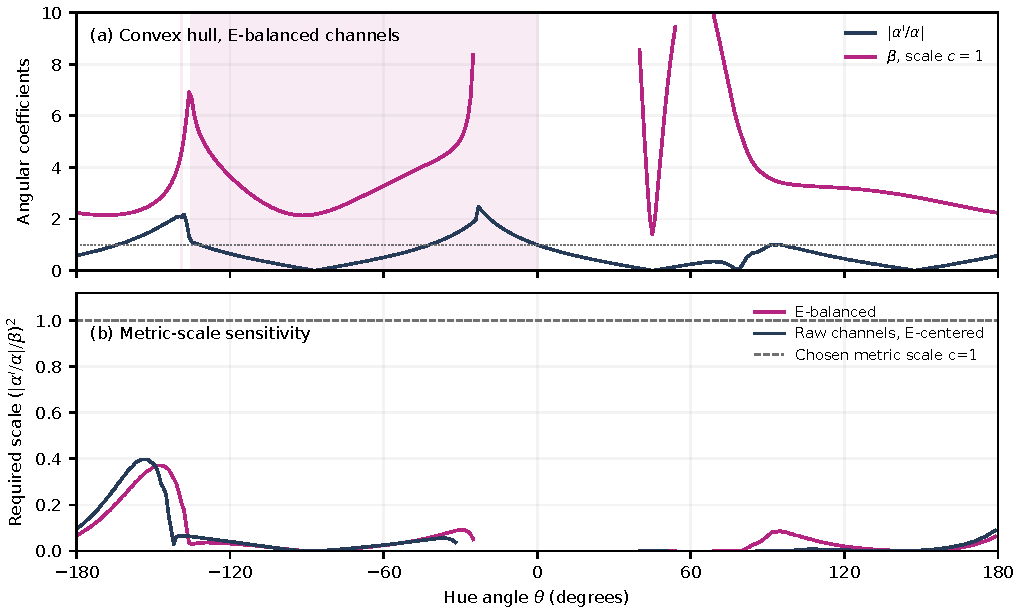
\includegraphics[width=0.94\textwidth]{fisher_bound_convex_hull.pdf}
\caption{Numerical compatibility for the convex hull of the selected 390--700~nm response vectors. (a) E-balanced profiles of $u=|\alpha'/\alpha|$ and the fixed-radius Fisher scale $\beta$; the dotted line marks the Euclidean reference $\beta=1$. Pink shading marks hull edges joining nonadjacent sampled wavelengths, not a perceptual hue class. (b) Required metric scales $(u/\beta)^2$ in both normalizations. The curves use a $1^\circ$ grid; Table~\ref{tab:bound} uses denser open-edge samples. Values with $\beta\geq10$ are omitted from the $\beta$ trace and panel (b). The filter and metric scale are modeling choices. The vector figure was generated with Matplotlib 3.10.8 by Python code developed with OpenAI ChatGPT/Codex assistance; it contains calculated model quantities, not experimental measurements.}
\label{fig:numerical}
\end{figure*}

A control calculation explains why the boundary definition and differentiation method matter. On the original spectral-locus construction, a $1^\circ$ angular grid misses a narrow raw-normalization failure near 403~nm. Differentiating a PCHIP interpolation of the LMS functions resolves it: at 403.4~nm, $u\approx5.9852$ and $\beta\approx5.2312$, so $(u/\beta)^2\approx1.3091$. This feature is inside the attainable mixture hull and is therefore not a failure of the outer-boundary check in Table~\ref{tab:bound}. It is retained in the reproducibility archive to document why the coarse original-locus result cannot support an all-hue claim.

\subsection{Metric scale and a testable comparison}
Writing $u=|\alpha'/\alpha|$, a common rescaling $G\mapsto cG$ gives $\beta\mapsto\sqrt c\,\beta$. On a fixed retained finite grid, strict compatibility is equivalent to
\begin{equation}
 c>c_*:=\max_\theta\left(\frac{u(\theta)}{\beta(\theta)}\right)^2.
 \label{eq:scale}
\end{equation}
The value $c=1$ is a convention in this illustration, not a measured physiological calibration. Increasing it can turn a failure into a pass without changing the boundary. Thus the test is hue-coordinate covariant but not independent of discrimination-metric normalization. The two properties must not be conflated.

For the Euclidean spatial reference metric, $B=r^2$ and $\beta=1$ in the stated polar coordinate. Comparing $u$ with 1 is a comparison with that specific metric. If the angle is reparameterized and the Euclidean tensor is transformed consistently, its comparison is covariant too. A failure of the fixed Euclidean benchmark does not, by itself, demonstrate a coordinate artifact or select the Fisher metric as physiological truth.

An empirical test would measure the ceiling and local discrimination independently in the same observer, stimulus class, adaptation state, coordinates, and units. It would propagate their uncertainties and fix the metric scale before evaluating the inequality. A large apparent margin obtained by comparing differently normalized metrics cannot supply that identification. In particular, the earlier manuscript's comparison with MacAdam ellipses \cite{MacAdam1942} did not resolve the scale and location mismatch between interior ellipse centers and boundary data; it is not used here as independent validation.

\section{Discussion}
\label{sec:discussion}
The model separates three questions that can otherwise become conflated. The first concerns hue organization: how an ordered spectral arc and a nonspectral purple arc enter a common cyclic target. The second concerns the representation of a chromatic body with an achromatic axis. The third concerns compatibility between a prescribed boundary and a calibrated indefinite metric. The first two motivate the coordinates of the third, but do not determine its metric signature or establish its physiological necessity.

The topological construction is deliberately modest. The compactification and insertion describe the target organization, not a new physical operation on electromagnetic wavelengths. The full cone of spectral stimuli already includes mixtures capable of inducing purples. Accordingly, nonspectrality does not pose an obstruction to physical causation. The explanatory task is to specify the response map and the viewing conditions under which its hue organization is represented by the proposed circle. A topological model by itself does not identify the relevant neural mechanism.

The metric calculation gives a conditional result with a definite mathematical content. Once the boundary form, the lack of temporal cross-terms, the calibration $C=\alpha^2$, and the angular coefficient $B$ have been prescribed, Eq.~\eqref{eq:square} supplies a necessary inequality. In the diagonal ansatz, strict inequality is sufficient for finite positive boundary data and a local regular collar. The construction is flexible: it neither singles out a unique interior metric nor selects the angular metric from cone fundamentals. This limits what a successful numerical illustration can establish.

There are two distinct aspects of the ridge claim. Within the symmetric bicone, the ridge at $z=0$ is an exact feature of the assumed boundary. Proposition~\ref{prop:ridge} gives a broader obstruction to a smooth null radial envelope, but only under its stated hypotheses. Neither result shows that every empirical color solid must have an isoluminant ridge. A measured smooth maximum would challenge an everywhere-null description within this metric class; it would not challenge the observed existence of nonspectral hues or the achromatic quotient.

The reachability interpretation introduces another independent task. Altered adaptation can change color appearance \cite{Shevell2003,Fairchild2013}, and chimerical-color demonstrations motivate comparisons between ordinary and altered response regimes \cite{Churchland2005}. Those demonstrations do not measure the metric or establish the location of an exterior state in the coordinates used here. Reports of reddish green and yellowish blue under special viewing conditions \cite{Crane1983} address a related but distinct phenomenon and should not be treated as interchangeable evidence for every proposed chimerical state.

To test non-egress, an experiment or physiological model would need to identify admissible controls near the candidate boundary and determine whether outward velocities remain available. Equation~\eqref{eq:identity} makes clear why invoking a null normal cannot substitute for that task. A successful control model could support a reachability interpretation without making ordinary optical motion globally causal in the Lorentzian sense. The geometry would still organize the compatibility question rather than supply the biological control law.

The numerical illustration also has a restricted domain. It uses a standard observer, a finite wavelength cutoff, the convex hull of tabulated responses, and a modeled angular information metric. It does not evaluate a measured object-color solid, individual observer variation, the full luminosity dependence of discrimination, or a measured purple appearance boundary. Straight mixture edges are meaningful for the declared additive stimulus model; the absence of a monochromatic correlate does not imply that nonspectral gamut boundaries are undefined in color science.

The priority for further testing is therefore independent calibration. One should first fix the stimulus class and observer, reconstruct a boundary in declared coordinates, and measure the relevant local discrimination tensor on that boundary. Only then can a failure or success of Eq.~\eqref{eq:bound-intro} carry the intended empirical weight. Additional measurements of accessible control directions would address confinement separately. Keeping these tests separate makes the model's assumptions and possible failure modes explicit.

\section{Conclusion}
The magenta gap motivates a response-side description of hue closure that distinguishes physical spectral stimuli from the cyclic organization of color. Inserting a purple interval into an auxiliary compactified spectral arc gives a resolved hue circle; collapsing that circle at zero chromatic radius gives a color body with an achromatic axis. These constructions provide the setting for a proposed reachability metric, without determining its signature.

For a prescribed hue-dependent bicone and explicit metric calibration, nullity and positive spatial definiteness imply a coordinate-covariant bound on the angular variation of the ceiling. The diagonal realization requires strict inequality, while regular equality can occur with a radial--angular cross-term. Cone-fundamental calculations illustrate compatibility with a specified metric convention. Independent discrimination calibration and a model of admissible optical controls remain necessary to establish empirical boundary constraints and physiological confinement.

\appendix
\section{Scope of the regular extension}
\label{app:extension}
The local extension used after Theorem~\ref{thm:diagonal} is a statement about compact patches of an open boundary sheet. Extend the smooth positive boundary coefficients along a transverse collar coordinate. A positive lower bound for $1-u^2/\beta^2$ on the patch keeps $A$ finite. A partition of unity can join its spatial tensor to a regular Cartesian spatial tensor away from the boundary, because positive-definite matrices form a convex cone. Interpolate the positive coefficient $C$ separately. Cutoffs are chosen to vanish on a full neighborhood of the interior axis, so arbitrary angular dependence does not survive at $x=y=0$.

This is stronger than requiring a correction merely to be $O(r^2)$: $r^2f(\theta)$ need not be smooth in Cartesian coordinates for arbitrary $f$. It also avoids extending a formula involving $|z|$ through the equator as though that formula were smooth. Separate sheet collars are sufficient for the local boundary statement; a globally smooth realization across all other regions is an additional construction problem.

There is a direct obstruction at the achromatic boundary tips for nonconstant $\alpha$. Along the boundary, $C=\alpha(\theta)^2$. Approaching $(0,\pm T)$ at different hues gives different limits for the coefficient of $\dd z^2$. The stipulated calibration therefore does not generally extend continuously to those tips. The regular Cartesian core concerns the open interior axis, not the closure including the anisotropic achromatic poles. No global smoothness or removable-singularity claim at those poles is required for the local compatibility theorem.

\begin{backmatter}
\bmsection{Acknowledgments}
The original manuscript records the use of Claude Opus 4.8, Gemini 3.1 Deep Think, and GPT-5.5 Pro for mathematical and computational stress tests and feedback on structure and exposition. OpenAI ChatGPT/Codex assisted with the present condensation, audit, and revision of the numerical code (session of 28 September 2026). The numerical figure is generated by the accompanying Python script from the supplied cone-fundamental arrays; no synthetic experimental observations are introduced.
\bmsection{Disclosures}
The author is affiliated with Alpha Omega Lattice Corporation. No physiological or psychophysical measurements are reported in this article.
\bmsection{Data availability}
The cone-fundamental input arrays, calculation script, machine-readable results, and figure-generation code used in this revision accompany the manuscript in its reproducibility archive. The original project materials are available at \url{https://github.com/AlphaOmega-Institute/magenta-gap}. The revised archive identifies the normalization and numerical conventions used for the results reported here.
\end{backmatter}

\begin{thebibliography}{12}
\bibitem{Krantz1975} D. H. Krantz, ``Color measurement and color theory: I. Representation theorem for Grassmann structures,'' J. Math. Psychol. \textbf{12}, 283--303 (1975).
\bibitem{Resnikoff1974} H. L. Resnikoff, ``Differential geometry and color perception,'' J. Math. Biol. \textbf{1}, 97--131 (1974).
\bibitem{Shevell2003} S. K. Shevell, ed., \emph{The Science of Color}, 2nd ed. (Elsevier, 2003).
\bibitem{Fairchild2013} M. D. Fairchild, \emph{Color Appearance Models}, 3rd ed. (Wiley, 2013).
\bibitem{Bujack2022} R. Bujack, E. Teti, J. Miller, et al., ``The non-Riemannian nature of perceptual color space,'' Proc. Natl. Acad. Sci. USA \textbf{119}, e2119753119 (2022).
\bibitem{Stockman2000} A. Stockman and L. T. Sharpe, ``The spectral sensitivities of the middle- and long-wavelength-sensitive cones derived from measurements in observers of known genotype,'' Vision Res. \textbf{40}, 1711--1737 (2000).
\bibitem{Stockman1999} A. Stockman, L. T. Sharpe, and C. Fach, ``The spectral sensitivity of the human short-wavelength sensitive cones derived from thresholds and color matches,'' Vision Res. \textbf{39}, 2901--2927 (1999).
\bibitem{Rao1945} C. R. Rao, ``Information and the accuracy attainable in the estimation of statistical parameters,'' Bull. Calcutta Math. Soc. \textbf{37}, 81--91 (1945).
\bibitem{Amari2016} S.-I. Amari, \emph{Information Geometry and Its Applications} (Springer, 2016).
\bibitem{MacAdam1942} D. L. MacAdam, ``Visual sensitivities to color differences in daylight,'' J. Opt. Soc. Am. \textbf{32}, 247--274 (1942).
\bibitem{Churchland2005} P. M. Churchland, ``Chimerical colors: some phenomenological predictions from cognitive neuroscience,'' Philos. Psychol. \textbf{18}, 527--560 (2005).
\bibitem{Crane1983} H. D. Crane and T. P. Piantanida, ``On seeing reddish green and yellowish blue,'' Science \textbf{221}, 1078--1080 (1983).
\end{thebibliography}
\end{document}
